\documentclass{beamer}
\usepackage[utf8]{inputenc}
\usepackage{hyperref} 
\usepackage{pgfpages}
\usepackage{amsmath,amssymb,mathrsfs}
\setbeamertemplate{navigation symbols}{} % turns off navigation symbols at the bottom of slides
\usepackage{graphicx}
\usepackage{amsmath}
\usepackage{caption}
\usepackage{subcaption}
\usepackage[round]{natbib}

\newtheorem{proposition}{Proposition}

\begin{document}
    
\title{Optimal Taxation with Heterogeneous Rates of Return}
\author[Hoffman, Shourideh]{Nick Hoffman\inst{1} \and Ali Shourideh \inst{1}}\institute[ ]{\inst{1} Carnegie Mellon University}

\begin{frame}
\titlepage 
\end{frame}

\section{Introduction}
\begin{frame}
    \frametitle{Summary}

    \begin{itemize}
        \item Study optimal \textit{nonlinear} taxation of capital income when agents earn heterogeneous returns on entrepreneurial investment
        \item Assets: entrepreneurial technology with idiosyncratic return, risk-free bond (``investing'' and ``saving'')
        \item Assume individual investment outputs imperfect substitutes 
        \begin{itemize}
            \item Eliminates undesirable ``solution'' 
        \end{itemize}
        \item Static model: differential asset taxation 
        \begin{itemize}
            \item Optimal distortions on both types of assets hump-shaped 
            \item Tax on investing uniformly higher than saving 
            \item Distortions driven by \textit{aggregate} DRS, informational frictions 
        \end{itemize} 
        \item Dynamic model: broadly progressive taxes in IID model 
        \begin{itemize}
            \item Wedge on investing history dependent, wedge on saving not 
            \item Additional force governing distortions: self-insurance
        \end{itemize}
    \end{itemize}

\end{frame}

\begin{frame}
    \frametitle{Motivation}

    \begin{itemize}
        \item Thick tails in wealth distribution driven by capital income risk: \cite{benhabib2011distribution}, \cite{benhabib2019wealth} 
        \begin{itemize}
            \item Multiplicative effect, rather than additive
        \end{itemize}
        \item How should capital income, wealth be taxed? 
        \begin{itemize}
            \item Can tax capital income to redistribute from wealthy to poor 
            \item Efficiency: excessive capital taxation discourages investment and lowers output
        \end{itemize} 
        \item \cite{mirrlees1971exploration}: framework to consider redistribution/efficiency tradeoff in the presence of informational frictions 
    \end{itemize}

\end{frame}

\begin{frame}
    \frametitle{Literature Review}

    \begin{itemize}
        \item Positive capital income taxes with informational frictions: \cite{golosov2003optimal}, \cite{kocherlakota2005zero}, \cite{albanesi2006dynamic}
        \begin{itemize}
            \item Common rate of return, labor market considerations
        \end{itemize} 
        \item Optimal taxation of entrepreneurs: \cite{albanesi2006optimal}, \cite{scheuer2014entrepreneurial}
        \begin{itemize}
            \item Entrepreneurial returns dependent on effort
            \item Support for differential rates 
        \end{itemize}
        \item \cite{guvenen2019use}: welfare improvement with \textit{wealth} taxes in a similar model
        \item Heterogeneous returns: \cite{shourideh2014optimal}, \cite{gerritsen2020optimal}
    \end{itemize}

\end{frame}

\section{Static Model}
\begin{frame}
    \frametitle{Static Model: Households and Productivity}

    Households
    \begin{itemize}
        \item Continuum of households who differ in type \( \theta \), which determines both \textit{productivity}, and \textit{variety} of intermediate good
        \item Assume \( \theta\in\Theta=\left[ \underline{\theta}, \bar{\theta} \right] \), with CDF \( F(\theta) \), privately known by household
        \item Household can borrow/lend \( b \) at common rate \( R \)
        \item Household of type \( \theta \) can also invest \( k \) capital and produce \( \theta k \) of their variety of intermediate good 
        \begin{itemize}
            \item Sells to final good producer at price \( p(\theta) \) 
            \item Price-taker, so individual technologies are CRS
        \end{itemize}
    \end{itemize}

\end{frame}

\begin{frame}
    \frametitle{Static Model: Aggregate Production and Prices}

    
    \begin{itemize}
        \item Final good producer combines intermediate goods to produce final good using CES aggregation technology: 
        \begin{equation*}
            Y = \left(\int_{\Theta}\left[\theta k\left(\theta\right)\right]^{\frac{\varepsilon-1}{\varepsilon}}dF\left(\theta\right)\right)^{\frac{\varepsilon}{\varepsilon-1}} 
        \end{equation*} 
        \item \( \varepsilon>1 \) elasticity of substitution 
        \begin{itemize}
            \item Ensures that at optimal solution, all types will invest
        \end{itemize}
        \item From FG producer problem, prices are 
        \begin{equation*}
            p(\theta) = \left(\frac{Y}{\theta k\left(\theta\right)}\right)^{\frac{1}{\varepsilon}}
        \end{equation*}
    \end{itemize}

\end{frame}

\begin{frame}
    \frametitle{Static Model: Government}

    \begin{itemize}
        \item Government levies taxes on income from investing \( \theta k p(\theta) \) and saving \( Rb \) according to tax function \( T \)
        \item Taking \( T \) and \( p \) as given, household solves 
        \begin{equation*}
            \max_{k,b}\ u\left(w-k-b\right)+\beta u\left[\theta kp\left(\theta\right)+Rb-T\left(\theta kp,Rb\right)\right]
        \end{equation*} 
        \item Benevolent government chooses \( T \) to maximize social welfare: 
        \begin{equation}
            \max \int_{\Theta}U\left(\theta\right)dF\left(\theta\right) \label{eq:static_swf}
        \end{equation}
        subject to revenue requirements and household optimality 
    \end{itemize}

\end{frame}

\begin{frame}
    \frametitle{Static Model: Mechanism Design Problem}

    \begin{itemize}
        \item Following from \cite{mirrlees1971exploration}, can recast government's problem in terms of mechanism design
        \begin{itemize}
            \item Revelation Principle: direct mechanism
            \item Household reports \( \theta \) and receives allocations
        \end{itemize} 
        \item Objective same as in \eqref{eq:static_swf}
        \item Feasibility constraints: 
        \begin{align*}
            w&\ge\int_{\Theta}\left[c_{0}\left(\theta\right)+k\left(\theta\right)\right]dF\left(\theta\right) \\
            \left(\int_{\Theta}\left[\theta k\left(\theta\right)\right]^{\frac{\varepsilon-1}{\varepsilon}}dF\left(\theta\right)\right)^{\frac{\varepsilon}{\varepsilon-1}}&\ge\int_{\Theta}c_{1}\left(\theta\right)dF\left(\theta\right) 
        \end{align*}
    \end{itemize}

\end{frame}

\begin{frame}
    \frametitle{Static Model: Mechanism Design Problem}

    \begin{itemize}
        \item Additional constraints: incentive compatibility
        \begin{multline*}
            U\left(\theta\right)\ge\ln\left(c_{0}\left(\hat{\theta}\right)+k\left(\hat{\theta}\right)-\frac{\hat{\theta}k\left(\hat{\theta}\right)}{\theta}\right)+\beta\ln c_{1}\left(\hat{\theta}\right), \\  \forall\theta,\hat{\theta}\in\Theta
        \end{multline*}
        where 
        \begin{equation*}
            U\left(\theta\right)=\ln c_{0}\left(\theta\right)+\beta\ln c_{1}\left(\theta\right)
        \end{equation*} 
        \item Simplifying assumption: while the planner (government) cannot observe \( \theta \), the market for intermediate goods \textit{can}
        \item If type \( \theta \) claims to be of type \( \hat{\theta} \), they still receive price \( p\left( \theta \right) \)
    \end{itemize}

\end{frame}

\begin{frame}
    \frametitle{Static Model: Optimal Distortions}
    
    \begin{itemize}
        \item From household problem, wedges are 
        \begin{align*}
            \tau_k(\theta) &= 1-\frac{u^{\prime}\left(c_{0}\right)}{\beta u^{\prime}\left(c_{1}\right)\theta p\left(\theta\right)} \label{eq:static_tk} \\
            \tau_b(\theta) &= 1-\frac{u^{\prime}\left(c_{0}\right)}{\beta Ru^{\prime}\left(c_{1}\right)}
        \end{align*} 
        \item First and second partial derivatives of tax function \( T \) 
        \item Optimal \textit{distortions}, not necessarily optimal taxes
    \end{itemize}
    
\end{frame}

\begin{frame}
    \frametitle{Static Model: Optimal Distortions}

    \begin{itemize}
        \item Assume log utility. 
        \item From optimality conditions in social planner's problem, can state wedges as 
        \begin{align*}
            \tau_{k}&=\left(1+\frac{k}{c_{0}}\right)\left(1-\frac{R}{\theta p\left(\theta\right)}\right) \\
        \tau_{b}&=\frac{k}{c_{0}}\left(\frac{\theta p\left(\theta\right)}{R} - 1\right) 
        \end{align*} 
        \item Two key determinants: \( \frac{k}{c_0} \), and \( \frac{R}{\theta p(\theta)} \) 
        \item Both wedges nonnegative, and positive on interior of \( \Theta \)
        \item \( \frac{k}{c_0} \) pulls wedges upward, effect of \( \frac{R}{\theta p(\theta)} \) depends on \( \theta \)
    \end{itemize}

\end{frame}

\begin{frame}
    \frametitle{Static Model: Marginal Product}

    \begin{lemma} \label{lem:thetap}
        At optimum, \( R\le\theta p(\theta) \), with equality if and only if \( \theta\in\left\{ \underline{\theta},\overline{\theta}\right\}  \).
    \end{lemma}

    \begin{itemize}
        \item \( \theta p(\theta) \) is the \textit{societal} marginal product of capital at the optimum for type \( \theta \), which takes into account effect of \( k \) on \( p \)
        \item Using formula for prices, 
        \begin{equation*}
            \theta p(\theta) = \theta^{1-\frac{1}{\varepsilon}} \left(\frac{Y}{ k\left(\theta\right)}\right)^{\frac{1}{\varepsilon}}
        \end{equation*} 
        \( \implies \) diminishing returns in aggregate
        \item Full information: planner wishes to equate \( \theta p(\theta) \) with \( R \)
        \item Informational frictions prevent this, \( \frac{\theta p(\theta)}{R} \) hump-shaped instead 
        \item For high values of \( \theta \), this term pulls wedges towards zero
    \end{itemize}

\end{frame}

\begin{frame}
    \frametitle{Static Model: Positive Wedge on Investing}

    \begin{itemize}
        \item Consequence of Lemma: optimal distortions are positive on the interior of \( \Theta \)
        \item Intuition for \( \tau_k>0 \): planner distorts investment choice to prevent over-supply of variety \( \theta \) 
        \item Without uncertainty, these can be interpreted as Pigouvian taxes 
        \begin{itemize}
            \item Externality: when I scale up, I affect not only \( p(\theta) \), but also the \textit{entire} pricing schedule 
        \end{itemize}
        \item Counterfactual: if households monopolists, investment wedge is lower and often negative; planner corrects for under-supply of variety 
    \end{itemize}

\end{frame}

\begin{frame}
    \frametitle{Static Model: Differential Asset Taxation}

    \begin{proposition} \label{prop:tauk_bigger}
        \( \tau_{k}\left(\theta\right)\ge\tau_{b}\left(\theta\right) \), with equality if and only if \( \theta\in\left\{ \underline{\theta},\overline{\theta}\right\}  \).
    \end{proposition}
    \begin{itemize}
        \item Optimality of positive \( \tau_b \) stems directly from positive \( \tau_k \) 
        \begin{itemize}
            \item Endowment is perfectly fungible between the two vehicles
        \end{itemize}
        \item Larger \( \tau_k \): investing income is a signal of private information, savings income is not
    \end{itemize}
\end{frame}

\begin{frame}
    \frametitle{Static Model: Numerical Example (Dual Problem)}

    \begin{itemize}
        \item \( \theta \sim N(1.5, 0.2) \) truncated over \( \Theta =[1,2]\)
        \item \( \beta = 0.9 \), \( \varepsilon = 4 \), \( w = 1 \), \( R = 1.5 \)
        \item Optimal allocations: 
    \end{itemize}
    \begin{figure}[htbp]
        \centering
        \caption{Allocations in the Static Model}
        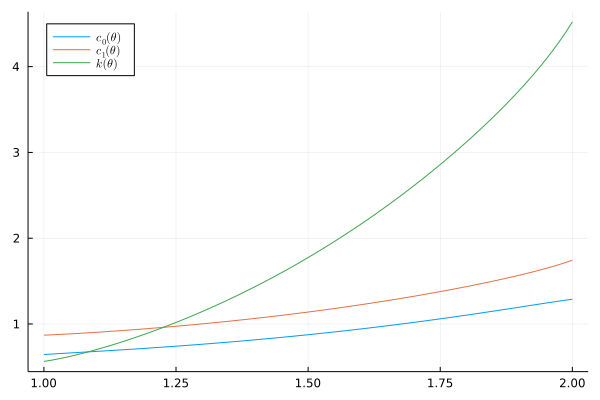
\includegraphics[width = 0.7\textwidth]{figures/static_allocs.png}
        \label{fig:static_allocs}
    \end{figure}

\end{frame}

\begin{frame}
    \frametitle{Static Model: Numerical Wedges}

    \begin{figure}[htbp]
        \centering
        \caption{Wedges in the Static Model}
        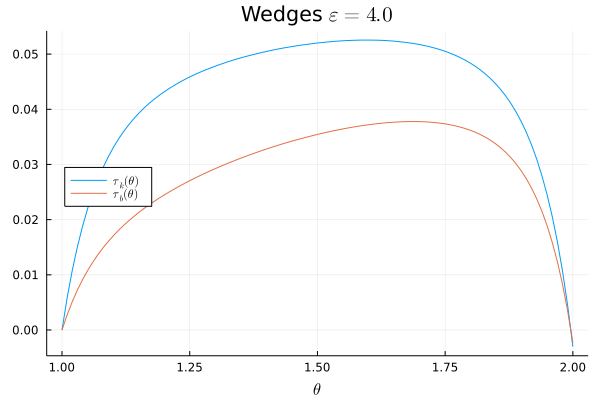
\includegraphics[width = 0.8\textwidth]{figures/static_wedges.png}
        \label{fig:static_wedges}
        % \caption*{\textit{Note: \( \theta^* \) denotes the value of \( \theta \) where the ratio \( \frac{\theta p\left( \theta \right)}{R} \) attains its maximum and begins to decline. This ratio is the force that ultimately pulls the wedges down.}}
    \end{figure}
    
\end{frame}

\begin{frame}
    \frametitle{Static Model: Determinants of Wedges}

    \begin{figure}[htbp]
        \centering
        \caption{Determinants of Wedges in the Static Model}
        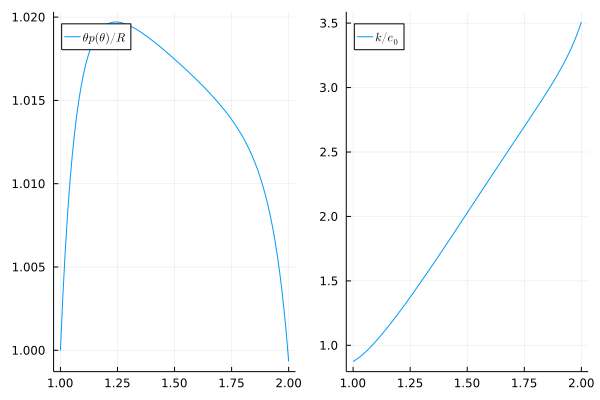
\includegraphics[width = 0.8\textwidth]{figures/static_determs.png}
        \label{fig:determs}
    \end{figure}
    

\end{frame}

\begin{frame}
    \frametitle{Static Wedges: Squeezing}

    \begin{figure}[htbp]
        \centering
        \caption{Squeezing Rates of Return: CDFs}
        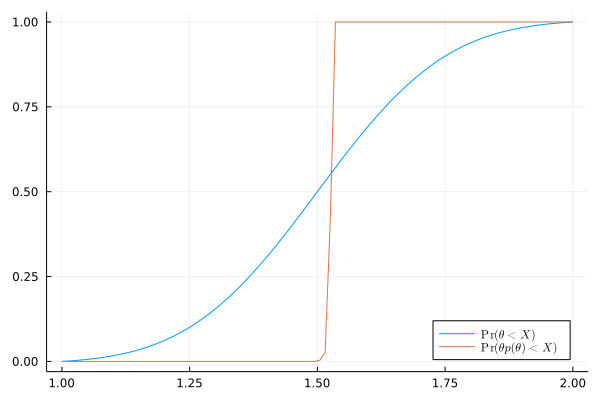
\includegraphics[width = 0.8\textwidth]{figures/static_cdfs.png}
        \label{fig:squeeze}
    \end{figure}

\end{frame}

\begin{frame}
    \frametitle{Static Model: Main Takeaways}

    \begin{itemize}
        \item Distortions driven by efficiency-equity tradeoff, informational rents, pricing concerns 
        \item \cite{farhi2010progressive}: distortions ``squeeze'' post-tax rates of return 
        \begin{itemize}
            \item Entrepreneurs price-takers \( \implies \) positive distortions
        \end{itemize}
        \begin{itemize}
            \item Variance in \( c_1 \) much smaller than variance in \( \theta \)
        \end{itemize}
        \item \cite{scheuer2014entrepreneurial}: intensive rather than extensive margin
        \begin{itemize}
            \item Rather than determining who selects into entrepreneurship, the tax code ensures that everyone invests the right amount 
        \end{itemize}
        \item Differential taxation: \( \tau_k > \tau_b \) on interior of \( \Theta \)
        \begin{itemize}
            \item Arbitrage, private information
        \end{itemize}
    \end{itemize}

\end{frame}

\begin{frame}
    \frametitle{Dynamic Model: IID Case}

    Production 
    \begin{itemize}
        \item Aggregate producer follows two-step process for \( Y_t \): 
        \begin{enumerate}
            \item Combines intermediate capital goods to create single capital good \( K_{t,f} \): 
            \begin{equation*}
                K_{t,f}=\left(\int\left[\theta_{t-1}k_{t}\left(\theta^{t-1}\right)\right]^{\frac{\varepsilon-1}{\varepsilon}}d\mu_{t-1}\left(\theta^{t-1}\right)\right)^{\frac{\varepsilon}{\varepsilon-1}}
            \end{equation*} 
            \item Combines \( K_{t,f} \) with labor \( L_t \), to produce \( Y_t \) according to Cobb-Douglas technology, \( Y_t = K_{t,f}^\alpha L_t^{1-\alpha} \)
        \end{enumerate}
        \item Assumption: \( L_t = L = 1 \ \forall t \), so final good output is 
            \begin{equation*}
                Y_t = K_{t,f}^\alpha
            \end{equation*}
            which ensures that a steady state in aggregates (\( Y,K_f \)) will exist
    \end{itemize}

\end{frame}

\section{Dynamic Model}
\begin{frame}
    \frametitle{Dynamic Model: IID Case}

    Households
    \begin{itemize}
        \item Time is discrete, each period plays out as follows: 
        \begin{enumerate}
            \item Agent realizes investing income 
            \begin{equation*}
                y_{t}\left(\theta^{t-1}\right)=p_{t}\left(\theta^{t-1}\right)\theta_{t-1}k_{t}\left(\theta^{t-1}\right)
            \end{equation*} 
            \item Agent draws new type \( \theta_t \) from \( F(\theta) \), draws IID across time. Then, agent makes choices \( c_t , k_t, b_t \)
        \end{enumerate} 
        \item Let $\theta^{t}=\left\{ \theta_{0},\theta_{1},...,\theta_{t}\right\} $ denote the history of shocks through time \( t \)
    \end{itemize}

\end{frame}

\begin{frame}
    \frametitle{Dynamic Model: IID Wedges}

    Wedges will be given by 
    \begin{align*}
        \tau_{k,t}\left(\theta^{t}\right)&=1-\frac{1}{\beta c_{t}\left(\theta^{t}\right)\theta_{t}p_{t+1}\left(\theta^{t}\right)\mathbb{E}\left[c_{t+1}\left(\theta^{t+1}\right)^{-1}\right]}\\\tau_{b,t}\left(\theta^{t}\right)&=1-\frac{1}{\beta c_{t}\left(\theta^{t}\right)R_t\mathbb{E}\left[c_{t+1}\left(\theta^{t+1}\right)^{-1}\right]}
    \end{align*}

\end{frame}

\begin{frame}
    \frametitle{Dynamic Model: Planning Problem}

    \begin{itemize}
        \item Let $\mu_{t}\left(\theta^{t}\right)$ denote the measure of period-$t$
        histories induced by the stochastic process for $\theta_{t}$. 
        \item The planner chooses allocations $\left\{ c_{t}\left(\theta^{t}\right),k_{t+1}\left(\theta^{t}\right)\right\} _{t=0}^{\infty}$
        to solve 
        \begin{equation}
        \max\sum_{t=0}^{\infty}\beta^{t}\int u\left(c_{t}\left(\theta^{t}\right)\right)d\mu_{t}\left(\theta^{t}\right)\label{eq:dyn_plan}
        \end{equation} 
        \item Feasibility assumes entrepreneurs allocated capital share \( \alpha Y\):
        \begin{align*}
            \int\left[c_{t}\left(\theta^{t}\right)+k_{t+1}\left(\theta^{t}\right)\right]&d\mu_{t}\left(\theta^{t}\right) \\ = \alpha&\left(\int\left[\theta_{t-1}k_{t}\left(\theta^{t-1}\right)\right]^{\frac{\varepsilon-1}{\varepsilon}}d\mu_{t-1}\left(\theta^{t-1}\right)\right)^{\frac{\alpha\varepsilon}{\varepsilon-1}} \\
            = \int&\theta_{t-1}p_{t}\left(\theta^{t-1}\right)k_{t}\left(\theta^{t-1}\right)d\mu_{t-1}\left(\theta^{t}\right)
        \end{align*}
    \end{itemize}

\end{frame}

\begin{frame}
    \frametitle{Dynamic Model: Incentive Constraints}

    \begin{itemize}
        \item Promise utility allocated to an agent of history $\theta^{t}$ is
        \begin{equation*}
        w_{t+1}\left(\theta^{t}\right)=\sum_{s=t+1}^{\infty}\beta^{s-t-1}\int u\left(c_{s}\left(\theta^{s}\right)\right)d\mu_{s}\left(\theta^{s}\big|\theta^{t}\right)
        \end{equation*} 
        \item The \textit{local} incentive constraints require 
        \begin{equation*}
            \frac{\partial U_t \left( \theta^t \right)}{\partial \theta_t}=u^{\prime}\left(c_{t}\left(\theta^{t}\right)\right)\frac{k_{t+1}\left(\theta^{t}\right)}{\theta_{t}}
        \end{equation*}
    \end{itemize}

\end{frame}

\begin{frame}
    \frametitle{Dynamic Model: Solving the Planning Problem}

    \begin{itemize}
        \item We focus on the dual (cost-minimization) problem of a \textit{component} planner 
        \begin{itemize}
            \item Considers the problem of a single agent of history \( \theta^{t-1} \)
            \item Takes the path of prices \( \left\{ p_{s+1}\left( \theta^s \right) \right\}_{s\ge t} \) as given 
        \end{itemize}
    \end{itemize}

\end{frame}

% \begin{frame}
%     \frametitle{Dynamic Model: Component Planner's Problem}
    
%     \begin{multline*}
%         \min_{\substack{c_{\tau}\left(\theta^{\tau}\right),k_{\tau+1}\left(\theta^{\tau}\right),\\
%         U_{\tau}\left(\theta^{\tau}\right),w_{\tau+1}\left(\theta^{\tau}\right)
%         }
%         }\sum_{\tau=t}^{\infty}\left(\prod_{s=t}^{\tau-1}R_{s}\right)^{-1} \left\{ \int\left[c_{\tau}\left(\theta^{\tau}\right)+k_{\tau+1}\left(\theta^{\tau}\right)\right]d\mu_{\tau}\left(\theta^{\tau}\right)- \right.
%         \\ \left. \int p_{\tau}\left(\theta^{\tau-1}\right)\theta_{\tau-1}k_{\tau}\left(\theta^{\tau-1}\right)d\mu_{\tau-1}\left(\theta^{\tau-1}\right) \right\}
%     \end{multline*}
%     subject to 
%     \begin{align*}
%         w_{t}\left(\theta^{t-1}\right) & =\sum_{\tau=t}^{\infty}\beta^{\tau-t}\int u\left[c_{\tau}\left(\theta^{\tau}\right)\right]d\mu_{\tau}\left(\theta^{\tau}\right)\\
%         U_{\tau}\left(\theta^{\tau}\right) & =u\left[c_{\tau}\left(\theta^{\tau}\right)\right]+\beta w_{\tau+1}\left(\theta^{\tau}\right)\\
%         \frac{\partial U_{\tau}\left(\theta^{\tau}\right)}{\theta_{\tau}} & =\frac{k_{\tau+1}\left(\theta^{\tau}\right)}{\theta_{\tau}c_{\tau}\left(\theta^{\tau}\right)}
%     \end{align*}
%     given \( p_{\tau}\left(\theta^{\tau-1}\right) \) and \( R_s \)
    
% \end{frame}

\begin{frame}
    \frametitle{Dynamic Model: Exploiting Homogeneity}

    \begin{itemize}
        \item Although the aggregate value function (cost-minimization) is not homogeneous, the component value function \textit{is}, as we assume that the CP takes prices as given 
        \begin{itemize}
            \item Similar to \cite{angeletos2007uninsured} 
        \end{itemize} 
        \item This allows us to derive a recursive formulation 
        \item Implies that the policy function for \( k_{t+1}\left( \theta^t \right) \) can be written as 
        \begin{align*}
            k_{t+1}\left(\theta^{t}\right) & =\overline{k}_{t+1}\left(\theta_{t}\right)\exp\left[\left(1-\beta\right)w_{t}\left(\theta^{t-1}\right)\right]\\
             & =\overline{k}_{t+1}\left(\theta_{t}\right)\exp\left[\left(1-\beta\right)\left(w^{\prime}\left(\theta_{t-1}\right)+...+w^{\prime}\left(\theta_{0}\right)+w_{0}\right)\right]
            \end{align*}
            for some functions \( \overline{k}\left( \theta_t \right) \) and \( w^\prime\left( \theta_t \right) \), in the case of log utility
    \end{itemize}

\end{frame}

\begin{frame}
    \frametitle{Dynamic Model: Exploiting Homogeneity}

    \begin{itemize}
        \item This decomposition implies a similar process for prices: 
        \begin{equation*}
            p_{t+1}\left(\theta^{t}\right)=\overline{p}_{t}\left(\theta^{t-1}\right)\hat{p}_{t}\left(\theta_{t}\right)
        \end{equation*}
        \item Can decompose price into \( \overline{p} \), which encodes history, and \( \hat{p} \), which only depends on \( \theta_t \)
        \item ``Common price'' \( \overline{p} \) evolves according to 
        \begin{equation*}
            \overline{p}_{t+1}\left(\theta^{t}\right)=\overline{p}_{t}\left(\theta^{t-1}\right)\tilde{p}\left(\theta_{t}\right)
        \end{equation*} 
        where 
        \begin{equation*}
            \tilde{p}\left(\theta_t\right)=\exp\left[-\frac{\left(1-\beta\right)}{\varepsilon}w^{\prime}\left(\theta_t\right)\right]
        \end{equation*}
            
    \end{itemize}

\end{frame}

\begin{frame}
    \frametitle{Dynamic Model: Recursive Formulation}
    Assuming constant \( R \), the recursive problem is:
    \begin{align*}
        C(w,\overline{p})=\min_{\substack{c(\theta),k^{\prime}(\theta),\\
        w^{\prime}(\theta),U(\theta)
        }
        } & \int\left\{ c\left(\theta\right)+k^{\prime}\left(\theta\right)+R^{-1}\left[C\left(w^{\prime}\left(\theta\right),\overline{p}\cdot\tilde{p}\left(\theta\right)\right)- \right.\right.\\
        &\left.\left.\overline{p}\cdot\hat{p}\left(\theta\right)\theta k^{\prime}\left(\theta\right)\right]\right\} dF\left(\theta\right)\\
        & \text{subject to} \\
        w & \le  \int U(\theta)dF(\theta)\\
        U(\theta) & =u\left(c(\theta)\right)+\beta w^{\prime}(\theta)\\
        U^{\prime}(\theta) & =u^{\prime}\left(c(\theta)\right)\frac{k^{\prime}(\theta)}{\theta}
    \end{align*}
    
\end{frame}

\begin{frame}
    \frametitle{Dynamic Model: Exploiting Homogeneity Once More}

    \begin{proposition}
        \label{prop:vf_homog}Suppose $u(c)=\ln c$. Then, the component planner's problem has the following solution: 
        \begin{align*}
        C\left(w,\overline{p}\right) & =A\left(\overline{p}\right)e^{\left(1-\beta\right)w} & w^{\prime}\left(\theta,w,\overline{p}\right) & =w^{\prime}\left(\theta,\overline{p}\right) + w \\
        c\left(\theta,w,\overline{p}\right) & =c\left(\theta,\overline{p}\right)e^{\left(1-\beta\right)w} & U\left(\theta,w,\overline{p}\right) & =U\left(\theta,\overline{p}\right)+w\\
        k^{\prime}\left(\theta,w,\overline{p}\right) & =k^{\prime}\left(\theta,\overline{p}\right)e^{\left(1-\beta\right)w}
        \end{align*}
        for some functions $A\left(\overline{p}\right),c(\theta,\overline{p}),k^{\prime}(\theta,\overline{p}),w^{\prime}(\theta,\overline{p}),U(\theta,\overline{p})$. 
    \end{proposition}
    
    \begin{itemize}
        \item Implication: we can solve the above problem for \( w=0 \) to obtain ``baseline'' functions $A\left(\overline{p}\right),c(\theta,\overline{p}),k^{\prime}(\theta,\overline{p}),w^{\prime}(\theta,\overline{p}),U(\theta,\overline{p})$. 
    \end{itemize}

\end{frame}

% \begin{frame}
%     \frametitle{Dynamic Model: Full Solution}
    
%     \begin{itemize}
%         \item The ``baseline'' functions solve the following recursion: 
%         \begin{multline*}
%             A\left(\overline{p}\right)=\min_{\substack{c(\theta),k^{\prime}(\theta),\\
%             w^{\prime}(\theta),U(\theta)
%             }
%             } \\ 
%             \int\left[c\left(\theta\right)+k^{\prime}\left(\theta\right)+R^{-1}\left\{ A\left(\overline{p}\cdot\tilde{p}\left(\theta\right)\right)\exp\left(\left(1-\beta\right)w^{\prime}(\theta)\right)- \right.\right.\\
%             \left.\left.\overline{p}\cdot\hat{p}\left(\theta\right)\theta k^{\prime}\left(\theta\right)\right\} \right]dF\left(\theta\right)
%         \end{multline*}
%         subject to 
%         \begin{align*}
%             0&=\int U(\theta,\overline{p})dF(\theta)\\U(\theta,\overline{p})&=\ln\left(c(\theta,\overline{p})\right)+\beta w^{\prime}(\theta,\overline{p})\\U^{\prime}(\theta,\overline{p})&=\frac{k^{\prime}(\theta,\overline{p})}{\theta c(\theta,\overline{p})}
%         \end{align*}
%     \end{itemize}
    
% \end{frame}

\begin{frame}
    \frametitle{Dynamic Model: Optimal Wedges}

    \begin{itemize}
        \item By definition, 
        \begin{equation*}
            \overline{p}_{t}\left(\theta^{t-1}\right)=\alpha K_{f}^{\alpha-1}K_{f}^{\frac{1}{\varepsilon}}\exp\left[-\frac{\left(1-\beta\right)}{\varepsilon}w_{t}\left(\theta^{t-1}\right)\right]  
        \end{equation*}
        \item In general equilibrium, there will be only one value of \( \bar{p} \) consistent with \( w=0 \), call this \( \bar{p}_0 \). 
        \begin{itemize}
            \item This is the value on which the ``baseline'' allocations are based.
            \item We still need to solve \( A\left( \bar{p} \right) \) for a range of \( \bar{p} \) values, but this value will not change from one period to the next 
        \end{itemize}
    \end{itemize}

\end{frame}

% \begin{frame}
%     \frametitle{Dynamic Model: Optimal Wedges}

%     \begin{itemize}
%         \item We can characterize the optimal wedges on saving and investing, respectively, as follows: 
%         \begin{align*}
%             \tau_{t+1,b}\left(\theta^{t+1}\right)&=1-\frac{c_{t+1}\left(\theta_{t+1}\right)\exp\left[\left(1-\beta\right)w_{t+1}\left(\theta_{t+1}\right)\right]}{\beta Rc_{t}\left(\theta_{t}\right)}\\
%             \tau_{t+1,k}\left(\theta^{t+1}\right)&=1-\frac{c_{t+1}\left(\theta_{t+1}\right)\exp\left[\left(1-\beta\right)w_{t+1}\left(\theta_{t+1}\right)\right]}{\beta c_{t}\left(\theta_{t}\right)\theta_{t}p_{t+1}\left(\theta^{t}\right)}
%         \end{align*} 
%         \item Prices are given by 
%         \begin{equation*}
%             p_{t+1}\left(\theta^{t}\right) =\alpha K_{f}^{\alpha-1}\left(\frac{K_{f}}{\theta_{t}k_{t+1}\left(\theta_{t}\right)e^{\left(1-\beta\right)w_{t}\left(\theta^{t-1}\right)}}\right)^{\frac{1}{\varepsilon}}
%         \end{equation*}
%     \end{itemize}

% \end{frame}

\begin{frame}
    \frametitle{Dynamic Model: Optimal Wedges}

    \begin{itemize}
        \item Thus, the optimal wedges will be given by the following: 
        \begin{align*}
            \tau_{k}\left(\theta,{\color{green}\bar{p}},w\right)&=1-\frac{\exp\left[\left(1-\beta\right)w^{\prime}\left(\theta,{\color{red}\bar{p}_{0}}\right)\right]}{\beta c\left(\theta,{\color{red}\bar{p}_{0}}\right){\color{green}\bar{p}}\hat{p}\left(\theta\right)\theta\mathbb{E}\left[c\left(\theta^{\prime},{\color{red}\bar{p}_{0}}\right)^{-1}\right]}\\\tau_{b}\left(\theta,{\color{green}\bar{p}},w\right)&=1-\frac{\exp\left[\left(1-\beta\right)w^{\prime}\left(\theta,{\color{red}\bar{p}_{0}}\right)\right]}{\beta Rc\left(\theta,{\color{red}\bar{p}_{0}}\right)\mathbb{E}\left[c\left(\theta^{\prime},{\color{red}\bar{p}_{0}}\right)^{-1}\right]}
        \end{align*}
        \item \( \tau_b \) independent of history, depends only on \( \theta_t \)
        \item \( \tau_k \) depends on \( \theta_t \), as well as history through \( {\color{green}\bar{p}} \)
    \end{itemize}

\end{frame}

\begin{frame}
    \frametitle{Dynamic Model: Optimal Wedges}

    Interpretation: Several Forces 
    \begin{itemize}
        \item For both \( \tau_b \) and \( \tau_k \) holding \( \bar{p} \) fixed, wedges will be closely related to their static counterparts
        \begin{itemize}
            \item In particular: correcting externalities 
            \item \( \tau_k \) will be increasing in \( \bar{p} \), so decreasing in promise utility \( w \)
        \end{itemize}
        \item There will be an additional force: household's insurance (consumption-smoothing) motive and its effect on incentive constraints. 
    \end{itemize}

\end{frame}

\begin{frame}
    \frametitle{Dynamic Model: Numerical Example}

    \begin{itemize}
        \item Can solve the recursive problem for \( A\left( \bar{p} \right) \) using the following parameterization: 
        \begin{align*}
            \beta&=0.9&\varepsilon&=4\\R&=1.1&\left\{ \underline{\theta},\overline{\theta}\right\} &=\left\{ 1,2\right\} \\\left\{ p_{H},p_{L}\right\} &=\left\{ 0,0.9\right\} &\theta&\sim N\left(1.5,0.2\right)
        \end{align*}
        \item Again assume that the distribution for \( \theta \) is truncated, only has support on \( \Theta \)
    \end{itemize}

\end{frame}

\begin{frame}
    \frametitle{Dynamic Model: Allocations}

    \begin{figure}[htbp]
        \centering
        \caption{Allocations in Infinite-Horizon Case}
        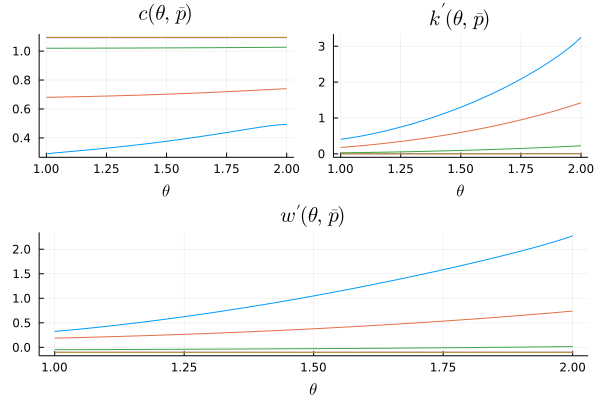
\includegraphics[width = 0.8\textwidth]{figures/inf_allocs_tnorm.png}
        \label{fig:inf_allocs}
    \end{figure}

\end{frame}

\begin{frame}
    \frametitle{Dynamic Model: Allocations}

    Main takeaway is the relationship of promised utility to the ``baseline'' allocations 
    \begin{itemize}
        \item Consumption \( c \) decreasing in \( \bar{p}_0 \), promise utility \( w^\prime \) increasing 
        \item Recall that \( \bar{p} \) and \( w \) move in opposite directions: lower \( \bar{p} \) \( \implies \) higher \( w \)
        \item Returns also increasing in \( \bar{p} \) 
        \item Upshot: consumption today \( c \) delivers on past promise, continuation promise utility \( w^\prime \) incentivizes current investment
    \end{itemize}

\end{frame}

\begin{frame}
    \frametitle{Dynamic Model: Rates of Return}

    \begin{figure}[htbp]
        \centering
        \caption{Rates of Return in Infinite-Horizon Case}
        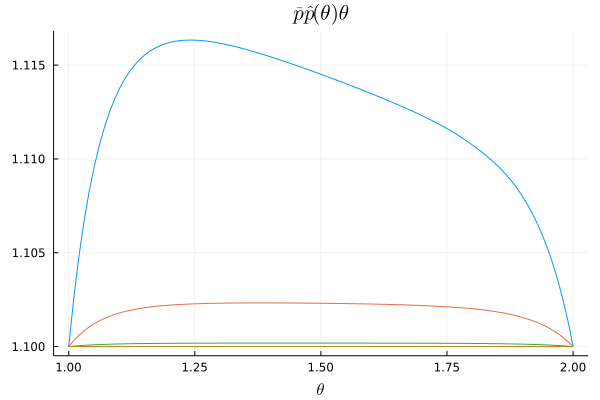
\includegraphics[width = 0.8\textwidth]{figures/inf_rors_tnorm.png}
        \label{fig:inf_rors}
    \end{figure}

\end{frame}

\begin{frame}
    \frametitle{Dynamic Model: Numerical Wedges}

    \begin{figure}[htbp]
        \centering
        \caption{Wedges in Infinite-Horizon Case}
        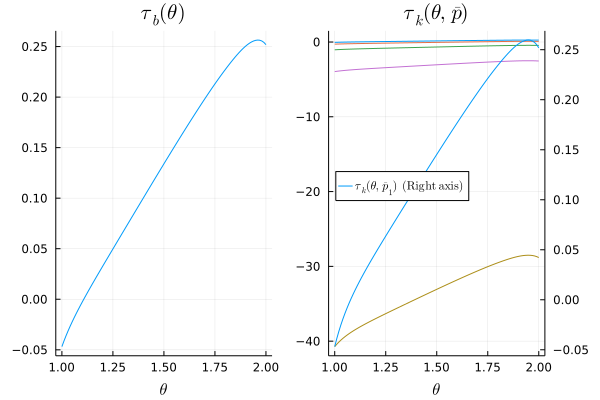
\includegraphics[width = 0.8\textwidth]{figures/inf_wedges_norm.png}
        \label{fig:inf_wedges}
    \end{figure}

\end{frame}

\begin{frame}
    \frametitle{Dynamic Model: Investing Wedge \( \tau_k \)}
    \begin{equation*}
        \tau_{k}\left(\theta,{\color{green}\bar{p}},w\right)=1-\frac{\exp\left[\left(1-\beta\right)w^{\prime}\left(\theta,{\color{red}\bar{p}_{0}}\right)\right]}{\beta c\left(\theta,{\color{red}\bar{p}_{0}}\right){\color{green}\bar{p}}\hat{p}\left(\theta\right)\theta\mathbb{E}\left[c\left(\theta^{\prime},{\color{red}\bar{p}_{0}}\right)^{-1}\right]}
    \end{equation*}
    \begin{itemize}
        \item \( \tau_k \) will depend on \( {\color{red}\bar{p}_{0}} \), \( {\color{green}\bar{p}} \), and \( \theta \)
        \item In general: will be increasing in \( \theta \) over most of the distribution (\textit{progressive})
        \item Slope and magnitude (and thus sign) will depend on \( {\color{red}\bar{p}_{0}} \) and \( {\color{green}\bar{p}} \)
        \item \textit{Generally speaking}: decreasing in  \( {\color{red}\bar{p}_{0}} \), increasing in \( {\color{green}\bar{p}} \) 
        \begin{itemize}
            \item Higher \( {\color{red}\bar{p}_{0}} \): less consumption, more \( w^\prime \) across all types 
            \item Higher \( {\color{green}\bar{p}} \): lower state (\( w \)), higher returns across all \( \theta \) (insurance motive again)
        \end{itemize}
    \end{itemize}

\end{frame}

\begin{frame}
    \frametitle{Optimal Capital Taxation: Dynamic Lessons}

    What do we make of these results? 
    \begin{itemize}
        \item Addition of uncertainty in dynamic context produces broadly progressive wedges
        \begin{itemize}
            \item Insurance motive: if I have a high type today, additional investing can tighten my incentive constraint tomorrow (I insure myself against a bad shock)
        \end{itemize}
        \item In both cases, taxation ``squeezes'' returns, as in \cite{farhi2010progressive} 
        \item Differential taxation result remains
        \item When returns driven by private information, optimal distortions are history-dependent 
        \begin{itemize}
            \item Possible role for taxation based on \textit{wealth}
        \end{itemize}
    \end{itemize}

\end{frame}


\section{Conclusion}
\begin{frame}
    \frametitle{Conclusion}

    \begin{itemize}
        \item Studied optimal nonlinear taxation of capital income with heterogeneous returns 
        \item Static model: positive, hump-shaped wedges 
        \begin{itemize}
            \item Investing income subject to strictly larger distortions than savings income 
        \end{itemize} 
        \item Dynamic model: derived recursive form, solved simplified planning problem 
        \begin{itemize}
            \item Investing wedge history-dependent and regressive in promise utility
            \item Savings wedge independent of history prior to \( t \) 
        \end{itemize}
    \end{itemize}

\end{frame}

% \begin{frame}
%     \frametitle{Remaining Work}

%     \begin{itemize} 
%         \item Static model: stochastic returns 
%         \item Infinite horizon: persistent shocks
%         \item Implementation in decentralized economy with taxes, transfers, and private borrowing/lending contracts 
%     \end{itemize}

% \end{frame}

\begin{frame}[allowframebreaks]
    \frametitle{References}

    \bibliographystyle{named}
    \bibliography{summer_paper_rg}

\end{frame}

\end{document}